%TODO: mejorar esto cuando esté más avanzado el TP y sepamos mejor qué escribir
\begin{abstract}
    En este trabajo se busca obtener un primer acercamiento al \'area de Procesamiento del Lenguaje Natural (NLP) y al análisis de sentimiento. Además se estudia el funcionamiento y efectividad del modelo de \textit{Bag of Words} (BoW) y las técnicas algorítmicas de k vecinos más cercanos (kNN) y el análisis de componentes principales (PCA) utilizados para la identificación de emociones en reseñas de películas.


	Por medio de experimentación intentaremos obtener el mejor análisis de sentimientos posibles. La calidad de los resultados de clasificación obtenidos será analizada mediante la métrica de accuracy.
\end{abstract}

\textit{Palabras clave:} bow, knn, pca, Sentiment Analysis, NLP

\begin{figure}[H]
    \centering
    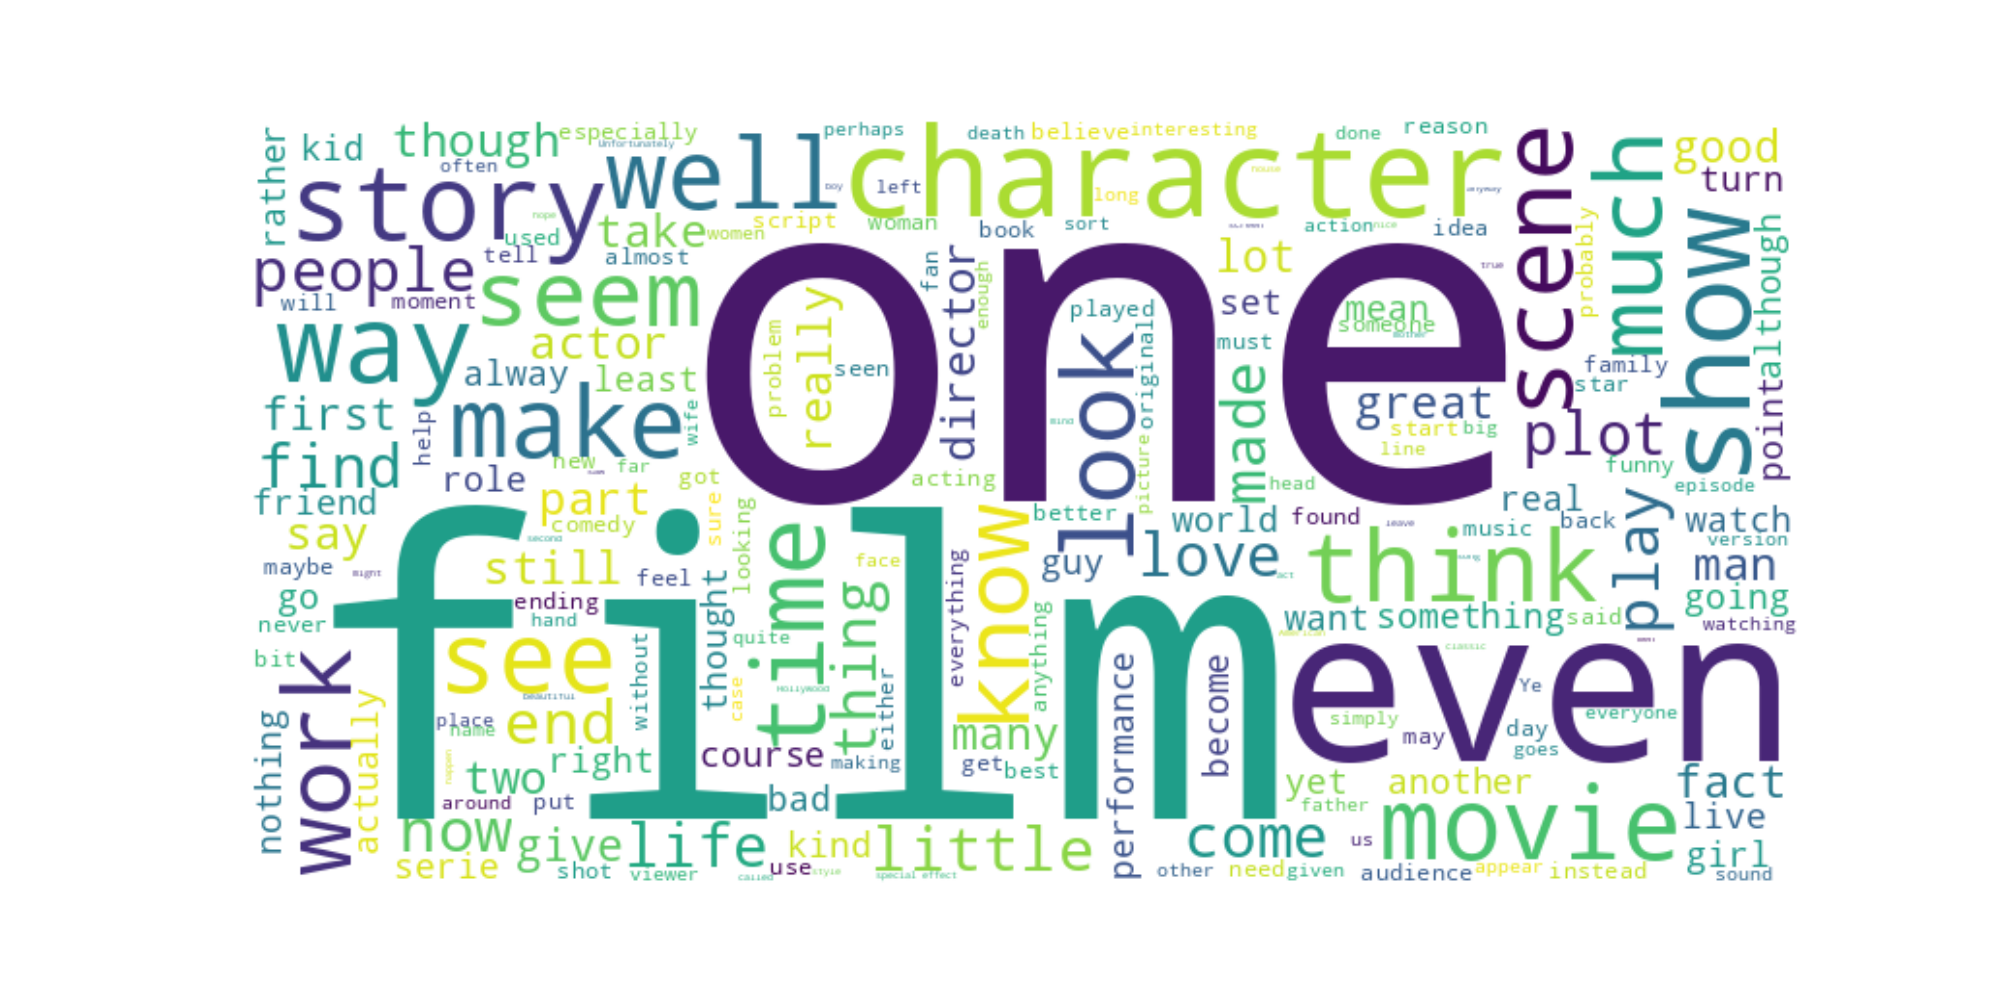
\includegraphics[ height=10cm, width=12cm]{../experimentos/wordcloud/wordcloud1.png}
    \caption{WordCloud armada con todas las palabras de las reviews}
\end{figure}
